\documentclass[12pt]{standalone}
\usepackage[svgnames]{xcolor}
\usepackage{tikz}
\usetikzlibrary{arrows.meta}\begin{document}
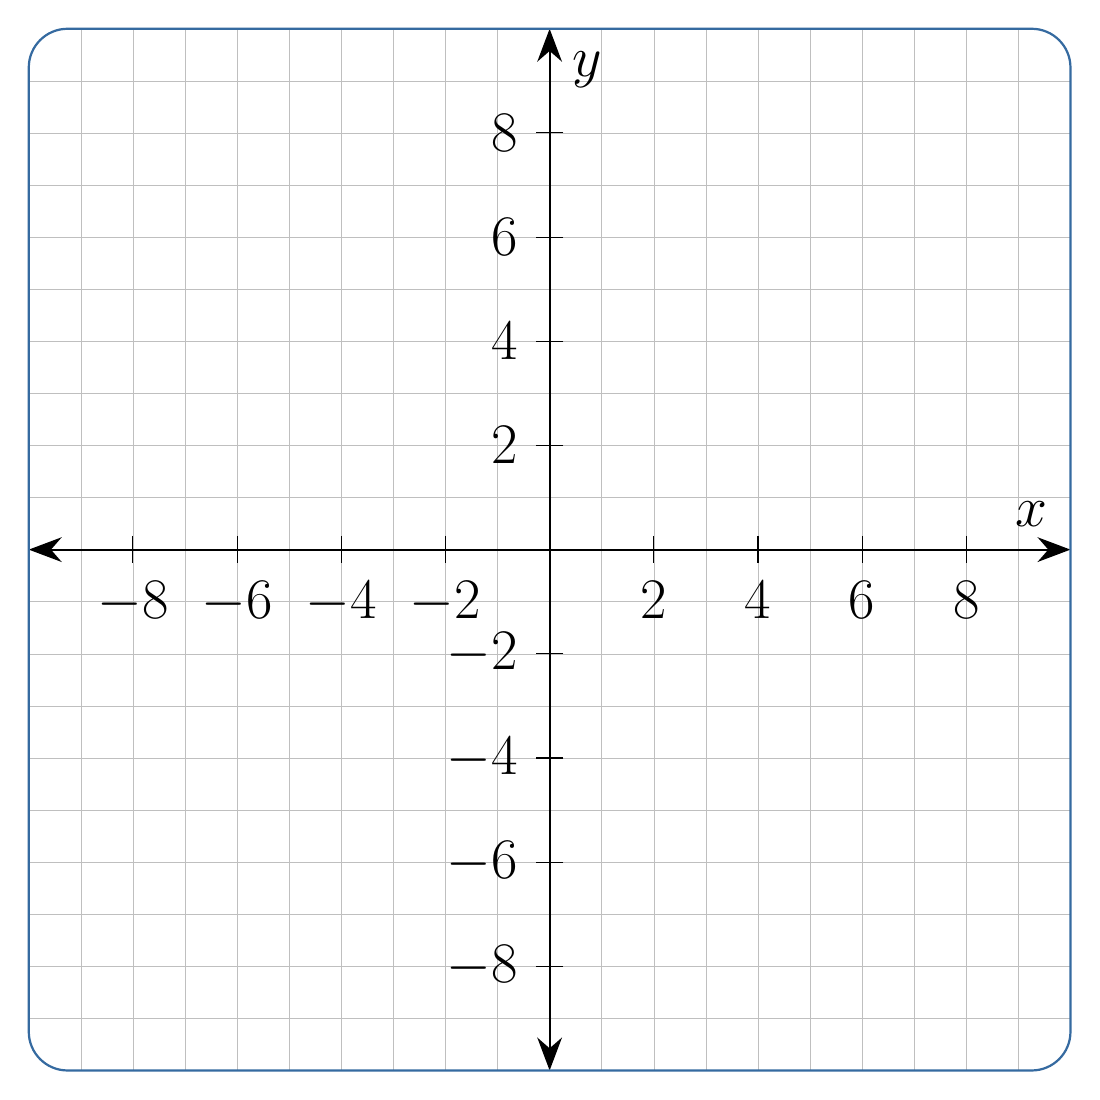
\begin{tikzpicture}[x=0.260416666666667in,y=0.260416666666667in]

\tikzset{
	>={Stealth[scale=1.8]},
	clip even odd rule/.code={\pgfseteorule},
	inverse clip/.style={ clip,insert path=[clip even odd rule]{
		(-10,-10) rectangle (10,10) }
	}
}
\definecolor{borderblue}{HTML}{356AA0}
\definecolor{fillpurple}{HTML}{A384E5}
\pgfdeclarelayer{background}
\pgfdeclarelayer{foreground}
\pgfsetlayers{background,main,foreground}
\begin{pgfonlayer}{background}
	\fill[white,rounded corners=14pt]
	(-10,-10) rectangle (10,10);
\end{pgfonlayer}
\foreach \x in {1,2,3,4,5,6,7,8,9,-1,-2,-3,-4,-5,-6,-7,-8,-9}{\draw[line width=0.2pt,color=lightgray] (\x,-10) -- (\x,10);}
\foreach \y in {1,2,3,4,5,6,7,8,9,-1,-2,-3,-4,-5,-6,-7,-8,-9}{\draw[line width=0.2pt,color=lightgray] (-10,\y) -- (10,\y);}
\huge
\draw[<->,thick] (-10,0) -- (10,0)
node[above left,outer sep=2pt]{\(x\)};
\draw[<->,thick] (0,-10) -- (0,10)
node[below right,outer sep=2pt]{\(y\)};
\foreach \x in {2,4,6,8,-2,-4,-6,-8}{\draw[thin] (\x,5pt) -- (\x,-5pt) node[below]{\(\x\)};}
\foreach \y in {2,4,6,8,-2,-4,-6,-8}{\draw[thin] (5pt,\y) -- (-5pt,\y) node[left]{$\y$};}
\draw[borderblue,rounded corners=14pt,thick] (-10,-10) rectangle (10,10);

\end{tikzpicture}
\end{document}
